
\begin{center}
\Huge
Prøve i diffentialregning
\end{center}
\begin{center}
Husk at skrive navn og sidetal på alle siderne. Sidetal skal skrives i formatet "Side $x$ af $y$" eller "$x/y$".\\
Prøven er uden hjælpemidler. I må benytte jer af jeres formelsamling, mine noter samt jeres egne noter.
\end{center}
\section*{Opgave 1}
En funktion $f$ er givet ved
\begin{align*}
f(x) = x^3 + \frac{4}{x}.
\end{align*}
\begin{enumerate}[label=\roman*)]
\item Differentiér funktionen $f$.
\item Bestem $f(2)$.
\item Bestem $f'(2)$.
\item Hvad er hældningen af tangenten for $f$ i punktet $(1,f(1))$?
\end{enumerate}
\section*{Opgave 2}
\begin{enumerate}[label=\roman*)]
\item Differentiér funktionen $f$ givet ved
\begin{align*}
f(x) = e^{x^2-4x+1}.
\end{align*}
\item Differentiér funktionen $g$ givet ved
\begin{align*}
g(x) = -2\ln(x)\sqrt{x}.
\end{align*}
\end{enumerate}
\section*{Opgave 3}
En funktion $f$ er givet ved 
\begin{align*}
f(x) = x^2+2x+1.
\end{align*}
\begin{enumerate}[label=\roman*)]
\item Bestem $f'(x)$.
\item Bestem en ligning for tangenten i punktet $(-2,f(-2))$.
\end{enumerate}
\section*{Opgave 4}
En funktion $f$ er givet ved
\begin{align*}
f(x) = \frac{1}{3}x^3-\frac{1}{2}x^2-2x+3.
\end{align*}
Grafen for funktionen $f$ fremgår af Fig. \ref{fig:fgraf}.
\begin{figure}[H]
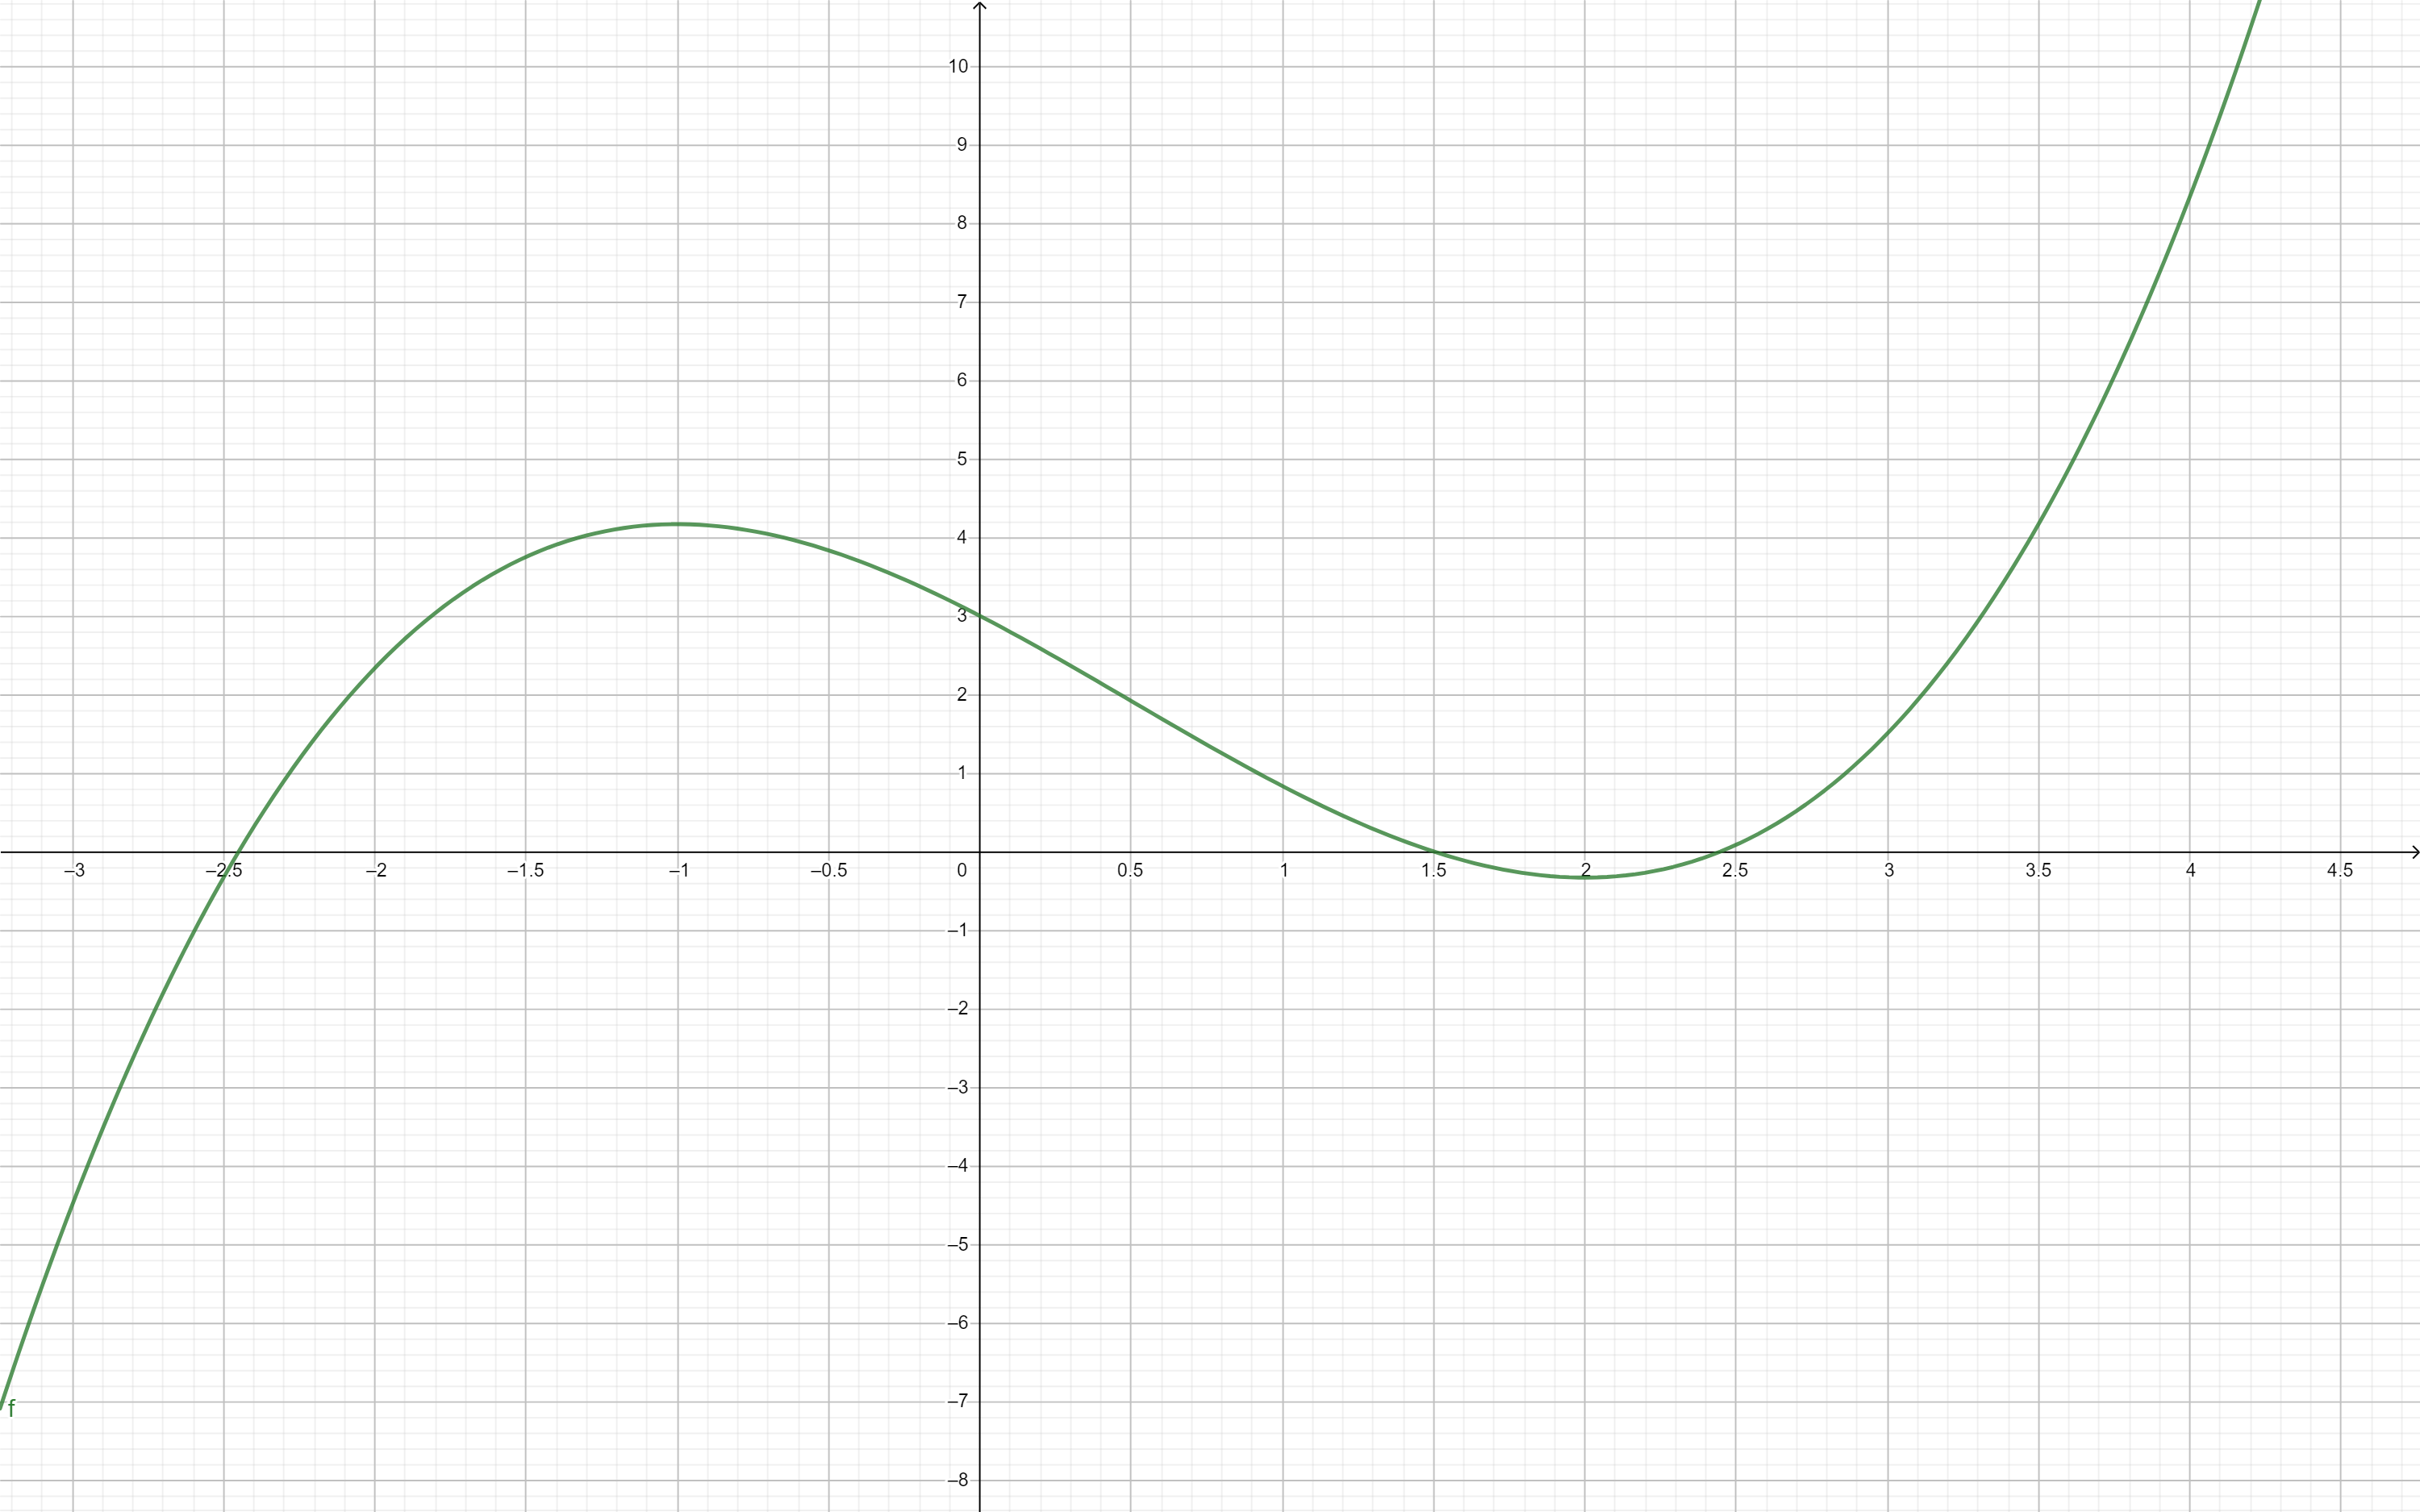
\includegraphics[width=\textwidth]{Billeder/toppunktsgraf}
\caption{Graf for funktionen $f$ på intervallet $-3<x<4,5$.}
\label{fig:fgraf}
\end{figure}
\begin{enumerate}[label=\roman*)]
\item Aflæs på Fig. \ref{fig:fgraf} hvor $f$ har ekstremumspunkter (maxima og minima).
\item Bestem $f'(x)$
\item Benyt $f'(x)$ til at bestemme ekstremumspunkterne eksakt.
\end{enumerate}